\documentclass[10pt]{beamer}

\usetheme{default}

\usepackage[utf8]{inputenc}
\usepackage[russian]{babel}
\usepackage[OT1]{fontenc}
\usepackage{amsmath}
\usepackage{amsfonts}
\usepackage{amssymb}
\usepackage{graphicx}
\usepackage{etoolbox}
\usepackage{caption}
\usepackage{subcaption}
\usepackage{pifont}
\usepackage{xcolor}
\usepackage{framed}
\definecolor{shadecolor}{cmyk}{0,0,0,1}
\usepackage{multirow}

\usepackage{listings}

\lstset{
	backgroundcolor=\color{lightgray},
	commentstyle=\color{blue},
	frame=single
	breakatwhitespace, 
	language=python, 
	columns=fullflexible, 
	keepspaces, 
	breaklines, 
	tabsize=3, 
	showstringspaces=false, 
	extendedchars=true,
	numbers=left
}

\makeatletter

\setbeamercolor{title}{fg=white}
\setbeamercolor{frametitle}{fg=black}
\setbeamerfont*{title}{family=\sffamily,size=\LARGE}

\setbeamerfont{page number in head/foot}{size=\scriptsize}
\setbeamertemplate{footline}[frame number]
\let\otp\titlepage
\renewcommand{\titlepage}{\otp\addtocounter{framenumber}{-1}}

\setbeamertemplate{background canvas}{%
	\ifnumequal{\c@framenumber}{0}{%
      
\includegraphics[width=\paperwidth,height=\paperheight]{images/cover.png}
   }{%
      \ifnumequal{\c@framenumber}{\inserttotalframenumber}{
         
\includegraphics[width=\paperwidth,height=\paperheight]{images/back.png}
      }{%
         % Other frames
      }%
   }%
}

\makeatother

\beamertemplatenavigationsymbolsempty

\author{Николай Анохин}
\title{\newline \newline \newline Лекция 6 \\ Линейные модели \\ для классификации и регрессии}

\begin{document}

\begin{frame}[plain]
\titlepage
\end{frame}

\begin{frame}{План занятия}
\tableofcontents
\end{frame}

\begin{frame}{Постановка задачи}

Пусть дан набор объектов $\mathcal{D} = \{(\mathbf{x}_i, y_i)\},
\; \mathbf{x}_i \in \mathcal{X},
\; y_i \in \mathcal{Y},
\; i \in 1, \ldots, N$, полученный из неизвестной закономерности $y = f(\mathbf{x})$. Необходимо выбрать из семейства параметрических функций
\[
H = \{h(\mathbf{x}, \theta): \mathcal{X} \times \Theta \rightarrow \mathcal{Y} \}
\]
такую $h^*(\mathbf{x}) = h(\mathbf{x}, \theta^*)$, которая наиболее точно апроксимирует $f(\mathbf{x})$.

\vspace{1em}
Задачи
\begin{itemize}
\item Регрессия: $\mathcal{Y} = [a, b] \subset \mathbb{R}$
\item Классификация: $|\mathcal{Y}| < C$
\end{itemize}

\end{frame}

% ============================================== %

\section{Линейная регрессия}

% ============================================== %

\begin{frame}{}

\begin{center}
\Large Линейная регрессия
\end{center}

\end{frame}

\begin{frame}{}

\begin{columns}[C]
    \begin{column}{.55\textwidth}
    	Модель
		\[
			y = h(\mathbf{x}, \theta) + \epsilon,
		\]
		где $\epsilon$ -- гауссовский шум
		\[
			\epsilon = \mathcal{N}(0, \beta^{-1}),
		\]
		откуда
		\[
		p(y | \mathbf{x}, \theta, \beta) = \mathcal{N}( h(\mathbf{x}, \theta), \beta^{-1})
		\]
    \end{column}
       
    \begin{column}{.45\textwidth}
	\begin{center}
   		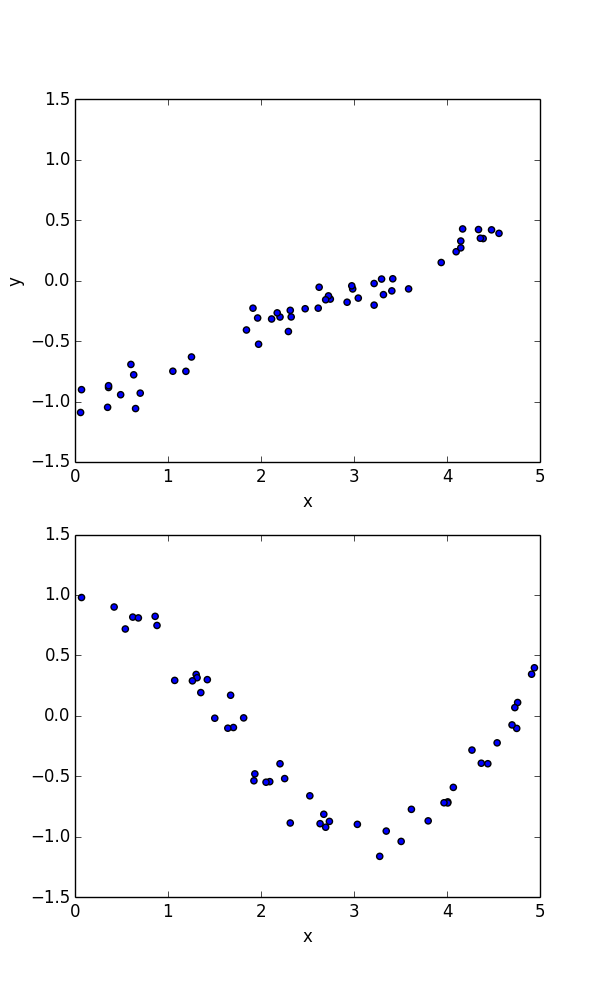
\includegraphics[scale=0.3]{images/empty_reg.png}
    \end{center}
    \end{column}
  \end{columns}

\end{frame}

\begin{frame}{Линейная модель}

\begin{columns}[C]
    \begin{column}{.55\textwidth}
    	простейшая модель
    	\[
    	y = w_0 + w_1 x_1 + \ldots + w_M x_M = \sum_{j=0}^M w_j x_j
    	\]
    	улучшенная модель
    	\[
    	y = \sum_{j=0}^M w_j \phi_j(\mathbf{x}),
    	\]
    	$\phi_j(\mathbf{x})$ -- базисная функция, $\phi_0(\mathbf{x}) = 1$
    \end{column}
       
    \begin{column}{.45\textwidth}
	\begin{center}
   		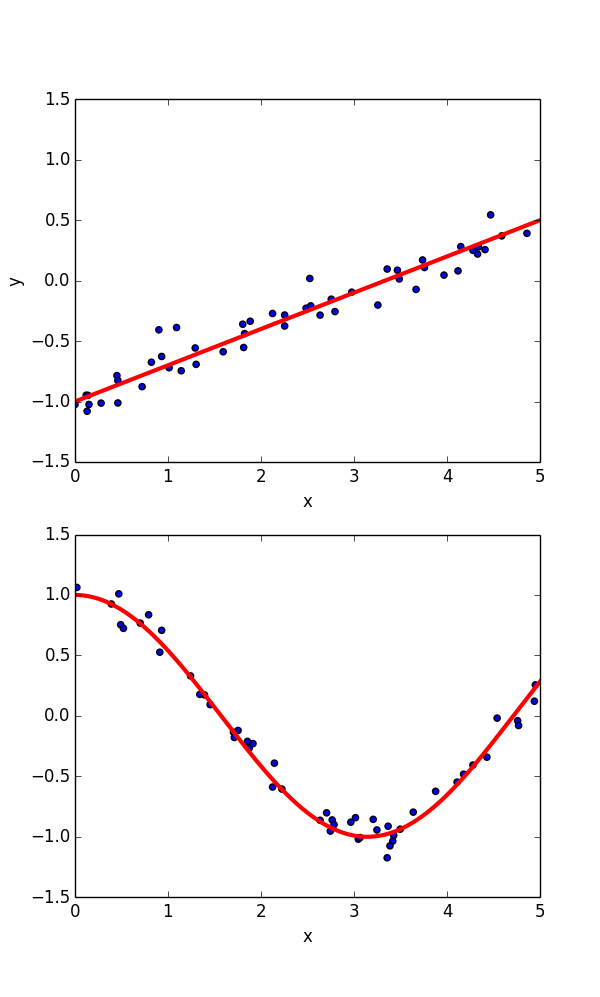
\includegraphics[scale=0.3]{images/full_reg.png}
    \end{center}
    \end{column}
  \end{columns}

\end{frame}

% ============================================== %

\section{Логистическая регрессия}

% ============================================== %

\begin{frame}{}

\begin{center}
\Large Логистическая регрессия
\end{center}

\end{frame}

% ============================================== %

\section{Обобщенные линейные модели}

% ============================================== %

\begin{frame}{}

\begin{center}
\Large Обобщенные линейные модели
\end{center}

\end{frame}

\begin{frame}{}

\begin{center}
\Large Вопросы
\end{center}

\end{frame}

\end{document}